\lecture{12}{2025-10-17}{Example of I/O/s and Exceptions}{}
Today's lecture is an example of what we did the previous weeks.
\begin{parag}{Parti 1a: Connecting an Input Peripheral}
	Consider an hypothetical processor with the following buses and control signals
	\begin{itemize}
		\item \texttt{A[31:1]} $\to $ Address bus 
		\item \texttt{D[31:1]} $\to $ Data bus 
		\item \texttt{AS} $\to $ Address Strobe (active when a valide address is present on \texttt{A[31:0]})
		\item \texttt{WR} $\to$ Write (active with an ASS when performing a write cycle)
	\end{itemize}
	\begin{subparag}{Bus protocol}
	\begin{center}
	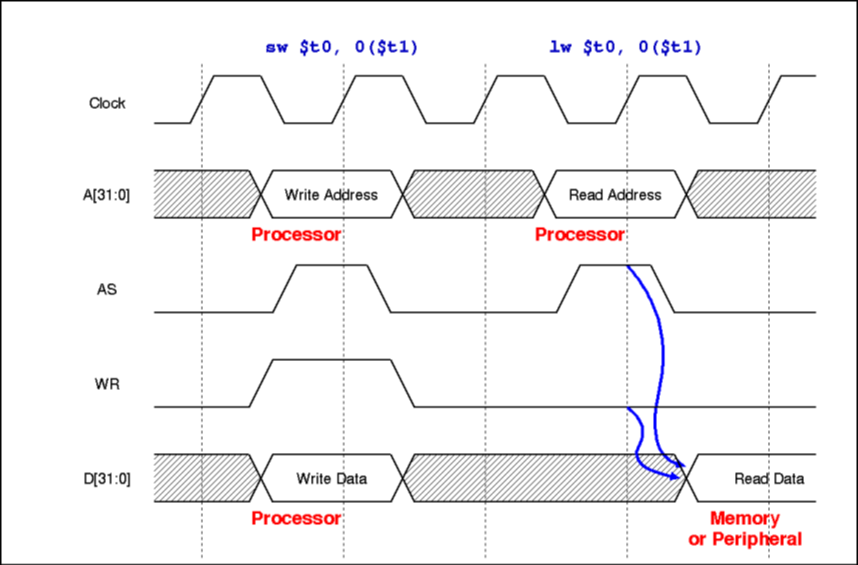
\includegraphics[scale=0.3]{screenshots/2025-10-17_3.png}
	\end{center}
    Here this is something that is very useful for us to read
	\end{subparag}
	\begin{subparag}{What do we want?}
	    \begin{itemize}
			\item Connect to the processor \important{10 buttons numbered from 0 to 9}
			\item Each button outputs a logic '1' if presse '0' otherwise 
			\item The processor must read the \important{state of the buttons} with a read from memory location \texttt{0xFFFF'FFF0}: '0' indicates no button pressed '1' indecates a button pressed 
			\item The processor must read the \important{number of the button pressed} with a read from memory location \texttt{0xFFFF'FFF4}.
	    \end{itemize}
	\end{subparag}
	The question now is: what do we need to do?\\
\end{parag}
\begin{parag}{Circuit}
    The first thing we need to do is to OR all the button together (so that if at least one of the button is pressed, the result woudd be one). Then we need to know which button is pressed. To do so, we need to decoode the buttons outputs into a 4 bits number $\implies $ we add a $2^n$ decoder. \\

	\begin{framedremark}
For the rest of the course I think the video is better than this because I cannot really explain it well while "drawing". 
	\end{framedremark}
\end{parag}


